\documentclass{beamer}

% \usetheme{Boadilla}
\usetheme{CambridgeUS}
\usecolortheme{dolphin}


% rus lang
\usepackage[main=russian,english]{babel}

% insert images
\usepackage{wrapfig}
\usepackage{graphicx}
\usepackage{float} % для позиционирования изображений
\usepackage{caption}
\captionsetup{format=hang,labelsep=period}
\graphicspath{{./images/}}

% tables
\usepackage{array} % расширенные возможности для работы с таблицами
\usepackage{tabularx} % автоматический подбор ширины столбцов
\usepackage{dcolumn} % выравнивание чисел по разделителю
\usepackage{{booktabs}}

% math
\usepackage{amsmath}
\usepackage{mathtools}
\usefonttheme[onlymath]{serif}
\newtheorem{rustheorem}{Теорема}

\newcommand{\at}[2][]{#1|_{#2}}
\newcommand{\eps}{\varepsilon}
\newcommand{\dd}[2]{\frac{\partial #1}{\partial #2}}

\DeclareMathOperator*{\argmin}{argmin}
\DeclareMathOperator{\sign}{sign}
\DeclareMathOperator{\K}{K}
% \DeclareMathOperator{\R}{\mathbb{R}}
\DeclareMathOperator{\X}{\mathbb{X}}
\DeclareMathOperator{\Y}{\mathbb{Y}}
% \DeclareMathOperator{\E}{\mathbb{E}}
\DeclareMathOperator{\V}{\mathbb{V}}

\newcommand{\E}[1]{\mathbb{E}\left[#1\right]} % Мат ожидание
\newcommand{\D}[1]{\mathbb{D}\left[#1\right]} % Дисперсия
\newcommand{\COV}[2]{Cov\left(#1, #2\right)}
\newcommand{\Cov}{\textbf{Cov}}
\newcommand{\R}{\mathbb{R}}
\renewcommand{\epsilon}{\varepsilon}
\renewcommand{\phi}{\varphi}
% algorithms
\usepackage[]{algorithm2e}

% \usepackage{cite} % поддержка цитирования
% \usepackage[hidelinks]{hyperref} % создание гиперссылок
% \usepackage{biblatex}


\title[]{ML для портфельной теории Марковица}
\subtitle{}
\author[Полузёров Т. Д.]{Полузёров Тимофей Дмитриевич}
% \institute[]{Научный руководитель Харин Алексей Юрьевич}
\date{}

\begin{document}
\begin{frame}
    \titlepage
\end{frame}

\begin{frame}
    \begin{center}
        \frametitle{Структура работы}
        \tableofcontents
    \end{center}
\end{frame}

\section{Портфельная теория}

\subsection{Постановка задачи}

\begin{frame}
    \frametitle{Однопериодная задача инвестирования}
    Доступны $N$ активов.
    $S_i^0, S_i^1$ --- цены $i$-го актива в моменты времени $t=0$ и
    $t=1$ соответственно.

    Доходность актива за период
    \[
        r_i := \frac{S_i^1 - S_i^0}{S_i^0}, i=\overline{1, N}
    \]

    Необходимо сформировать портфель
    \[
        b = (b_1, \dots, b_N)
    \]
    где $b_i$ --- число преобретаемых активов $i$-го типа.

    Портфель покупается в момент $t=0$ и продается в момент $t=1$ по рыночным ценам.
\end{frame}

\begin{frame}
    \frametitle{Доходность портфеля [4, 5, 6, 8]}
    Пусть инвестор имеет капитал $x$.

    Перейдем к долям инвестирования капитала $x$ в доступные активы.
    \[
        \omega_i := \frac{b_i S_i^0}{x}, i=\overline{1, N}
    \]

    Цена портфеля в момент времени $t=0$
    \[
        X^0 = x
    \]
    В момент $t=1$
    \[
        X^1 = (1+R)X^0 = \sum_{i=1}^{N} \omega_i r_i = \omega^T r
    \]
    где $R$ --- доходность порфтеля
\end{frame}

\begin{frame}
    \frametitle{Характеристики доходности портфеля}

    Предположим, что случайные величины доходностей $r_i, i=\overline{1, N}$ известны, тогда
    матожидание и дисперсия случайной величины доходности портфеля равны
    \[
        \mu_X := \E{R} = \sum_{i=1}^{N} \omega_i \E{r_i} = \omega^T \mu
    \]

    \[
        \sigma_X^2 := \sum_{i=1, j=1}^{N} \omega_i \omega_j \COV{r_i}{r_j} =
        \omega^T \Sigma \omega
    \]
    где $\mu = \E{r}$, а $\Sigma$ --- ковариационная матрица случайного вектора $r$.
\end{frame}

\begin{frame}
    \frametitle{Интерпретация характеристик доходости портфеля}
    \begin{figure}
        \centering
        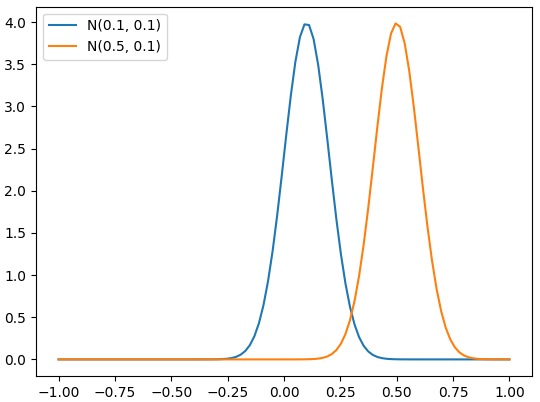
\includegraphics[width=0.75\textwidth]{equal_var_cut.png}
        \caption{Предпочтения в средней доходности портфеля}
        \label{fig:equal_var}
    \end{figure}
\end{frame}

\begin{frame}
    \frametitle{Дисперсия как мера риска}
    \begin{figure}
        \centering
        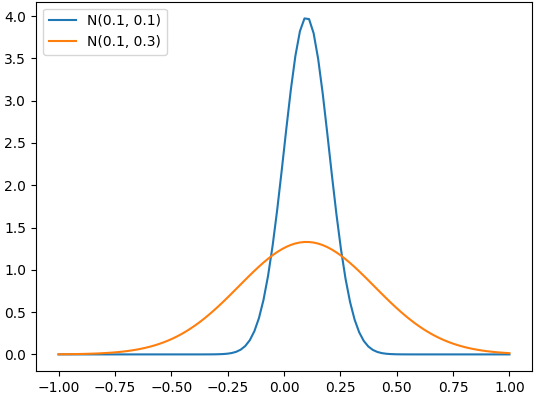
\includegraphics[width=0.75\textwidth]{equal_mean_cut.png}
        \caption{Предпочтения в риске портфеля}
        \label{fig:equal_mean}
    \end{figure}
\end{frame}

\subsection{Оптимизационная задача}

\begin{frame}
    \frametitle{Оптимизационная задача}
    Введем параметр $\tau \in [0, +\infty)$ --- толерантность к риску и сформурируем критерий оптимальности
    \[ 
        f(\mu_X, \sigma_X^2) = \tau \omega^T \Sigma \omega - \omega^T \mu \rightarrow \min_{\omega}
    \]

    Оптимизационная задача имеет вид
    \begin{align*}
        \begin{cases}
            \tau \omega^T \Sigma \omega - \omega^T \mu \rightarrow \min_{\omega} \\
            \omega^T e = 1 \\
            \omega \ge 0
        \end{cases}
    \end{align*}

    При $\tau=0$ имеем портфель максимальной доходности, при $\tau \rightarrow +\infty$
    --- минимального риска.
\end{frame}

% \subsection{Диверсификация}

% \begin{frame}
%     \frametitle{}

% \end{frame}

\section{Методы оценки характеристик доходностей}

\begin{frame}
    \frametitle{Подходы к оценке характеристик}

    На практике в момент времени $t=0$ случайные величины доходностей $r$ неизвестны.
    
    Необходимо оценить характеристики $\hat{\mu}_X$ и $\hat{\Sigma}$.

    Известные подходы:
    \begin{itemize}
        \item Модель CAPM (Capital Asset Pricing Model), У. Шарп, Дж Линтер [9, 13]
        \item Теория  APT (Arbitrage Pricing Theroy), С. Росс, Р. Ролл. [11, 12]
    \end{itemize}
    
    Предлагается иной подход --- применить методы машинного обучения и модели временных
    рядов для решения задачи регрессии по историческим данным.
\end{frame}

\subsection{Линейная регрессия}

\begin{frame}
    \frametitle{Линейная регрессия [1], [2]}
    Пусть $X$ --- матрица объектов-признаков, где признаки это лаги ряда,
    $y$ --- соотвествующие истинные доходности.
    $\theta = (\theta_0, \dots, \theta_k)$ --- параметры.
    
    \[
        a(x) = \theta_0 + \theta_1 x_1 + \dots + \theta_k x_k
    \]
    Оптмальные веса $\theta^*$ определяются методом наименьших квадратов
    \[
        Q(a) = || X\theta - y||^2 \rightarrow \min_{\theta}
    \]
\end{frame}

\subsection{Случайный лес}

\begin{frame}
    \frametitle{Случайный лес [2, 7]}

    Дерево решений --- это бинарное дерево.
    Вершины двух типов:
    \begin{itemize}
        \item внутренние --- содержат предикат $b_v: \mathbb{X} \rightarrow {0, 1}$
        \item листовые --- хранят выходное значение $c_v \in \mathbb{Y}$
    \end{itemize}

    Обработка входящего объекта $x$:
    \begin{enumerate}
        \item старт из корня
        \item вычисляем значение текущего предиката $b_v(x)$
        \item если значение $b_v(x) = 0$ делаем шаг в левое поддерево, иначе --- в правое
        \item пока не дошли до листа повторяем шаги 2 и 3
        \item возвращаем значение $c_v$ из текущего листа
    \end{enumerate}
\end{frame}

\begin{frame}
    \frametitle{Случайный лес [2, 7]}

    Случайный лес есть усреднение набора решающих деревьев
    \[
        a(x) = \frac{1}{k} \sum_{i=1}^{k} b_i(x)
    \]
    Среднеквадратичную ошибку можно разложить на слагаемые:
    \[
        Q(a) = bias(a) + variance(a) + noise
    \]
    где 
    \[
        bias(a) := f(x) - \mathbb{E}_X\left[a(x, X)\right]
    \]
    \[
        variance(a) := \mathbb{E}_X\left[a(x, X)\right] -\mathbb{E}_X\left[a(x, X)\right]^2
    \]
    \[
        noiсe := \mathbb{E}_X\left[\mathbb{E}_{\epsilon}\left[\left( y(x, \epsilon) - f(x) \right)^2\right]\right]
    \]
\end{frame}

\begin{frame}
    \frametitle{Случайный лес [2, 7]}

    Смещение композиции равно смещению базового алгоритма
    \begin{align*}
        bias(a) = bias_X(b)
    \end{align*}
    
    Разброс композиции определяеся размером композиции и коррелированностью базовых алгоритмов
    \begin{align*}
    	variance(a) =
         \frac{1}{k^2} \sum_{i=1}^{k} variance_X(b_i) + 
        \frac{1}{k^2} \sum_{i \ne j} \COV{b_i}{b_j}
    \end{align*}

\end{frame}

\subsection{ARIMA}

\begin{frame}
    \frametitle{ARIMA [5]}
    Модель $ARMA(p, q)$ объединяет модели авторегрессии $AR(p)$ и скользящего среднего $MA(q)$.
    \begin{align*}
        x_n = & \left(a_0 + a_1 x_{n-1} + \dots + a_p x_{n-p} \right) + \\
	    + & \left(b_1 \epsilon_{n-1} + b_2 \epsilon_{n-2} + \dots + b_q \epsilon_{n - q} \right) \\
        + & \sigma \epsilon_n
    \end{align*}
    где $\epsilon = (\epsilon_n)$ --- белый шум.

    Разности процесса
    \[
        \Delta x_n = x_n - x_{n-1}
    \]

    Символически $ARIMA(p, d, q)$ выражается через модель $ARMA(p, q)$
    \[
        \Delta^d ARIMA(p, d, q) = ARMA(p, q)
    \]
\end{frame}

\section{Проверка статегий на реальных данных}

\subsection{Обзор данных}

\begin{frame}
    \frametitle{Входные данные}
    Общие характеристики данных:
    \begin{itemize}
        \item Криптовалютная биржа OKX [3]
        \item 8 наиболее популярных активов
        \item Временной период с 1 января 2022 г. по 1 января 2025 г.
        \item Дневной таймфрейм
        \item Период инвестирования --- 1 неделя
    \end{itemize}

    Проведение тестирования:
    \begin{itemize}
        \item Данные до 1 января 2024 г. используются для подбора числа лагов и 
        гиперпараметров моделей
        \item Тестирование проводится на данных за 2024 год
    \end{itemize}
\end{frame}

\begin{frame}
    \begin{columns}
        \begin{column}{0.5\textwidth}
            \begin{figure}
                \centering
                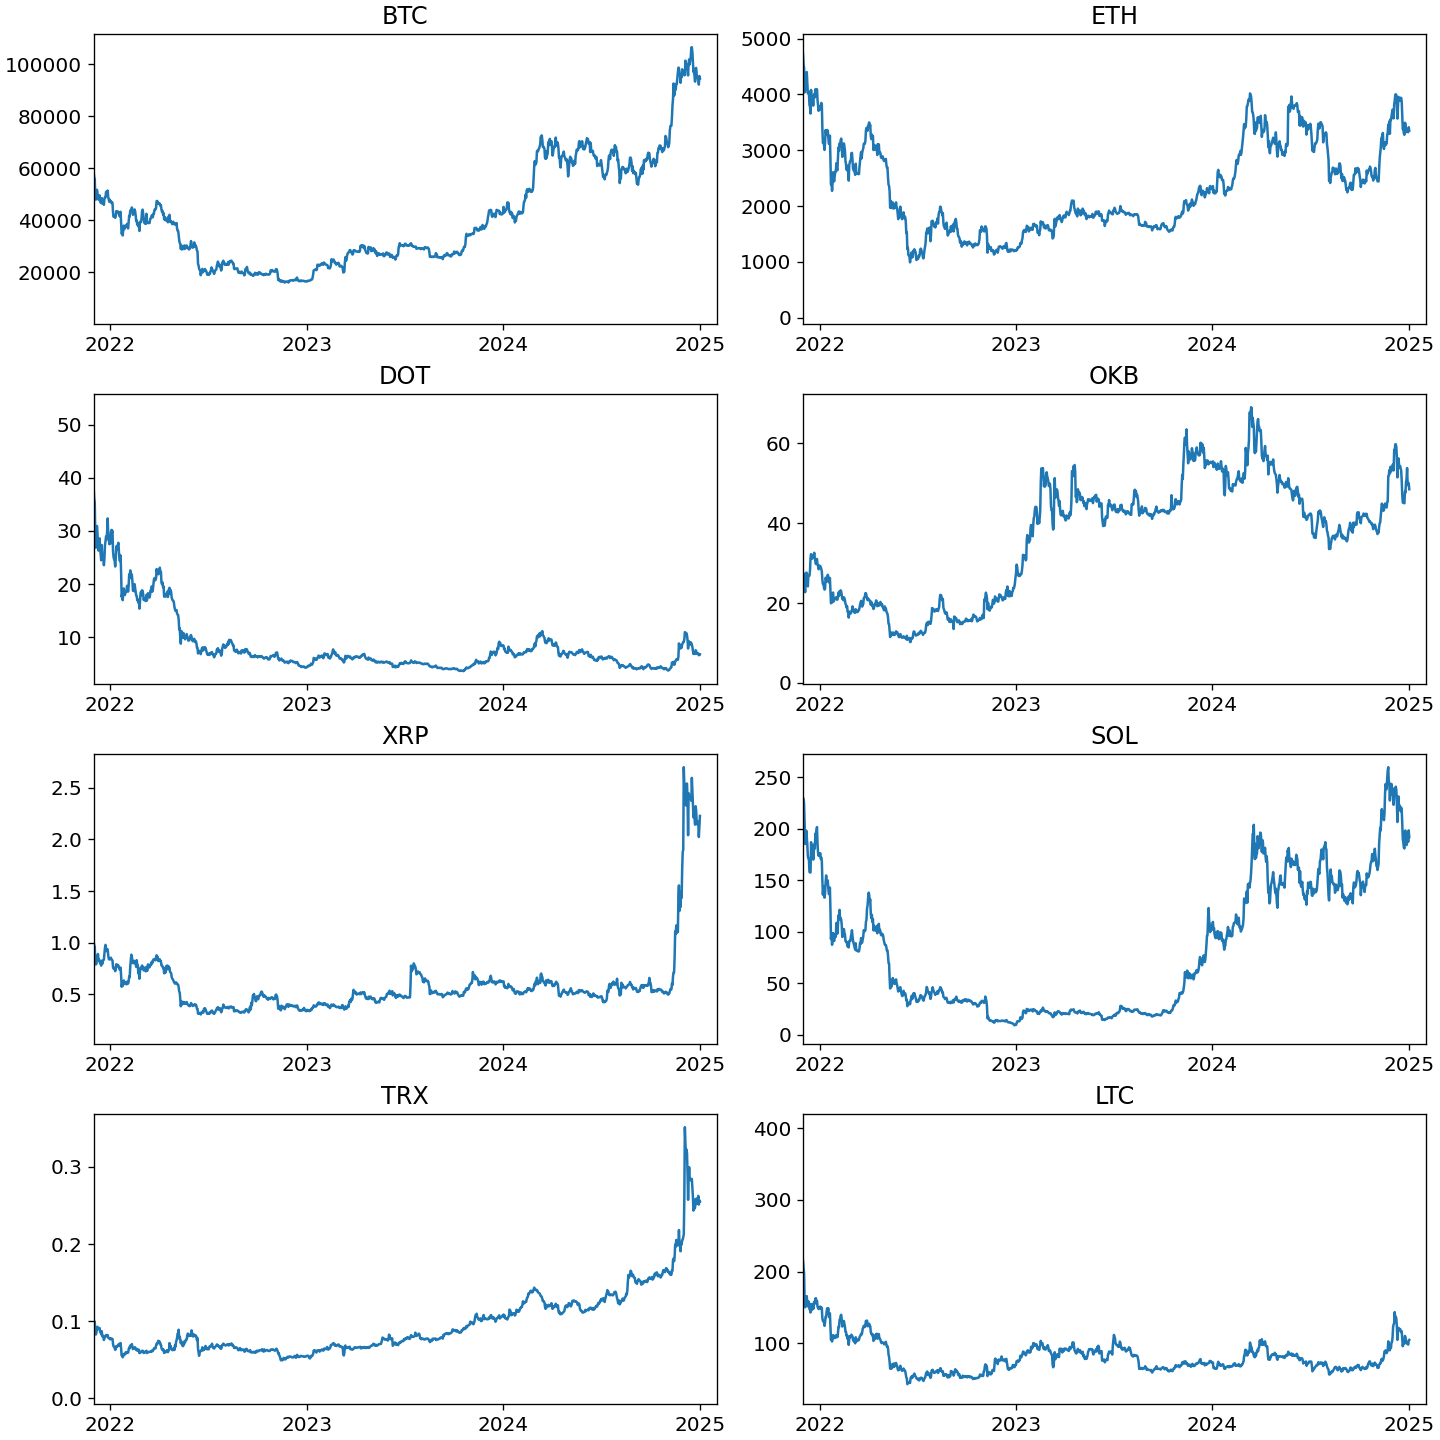
\includegraphics[width=1\textwidth]{prices.png}
                \caption{Цены активов}
                \label{fig:prices}
            \end{figure}
        \end{column}
        \begin{column}{0.5\textwidth}
            \begin{figure}
                \centering
                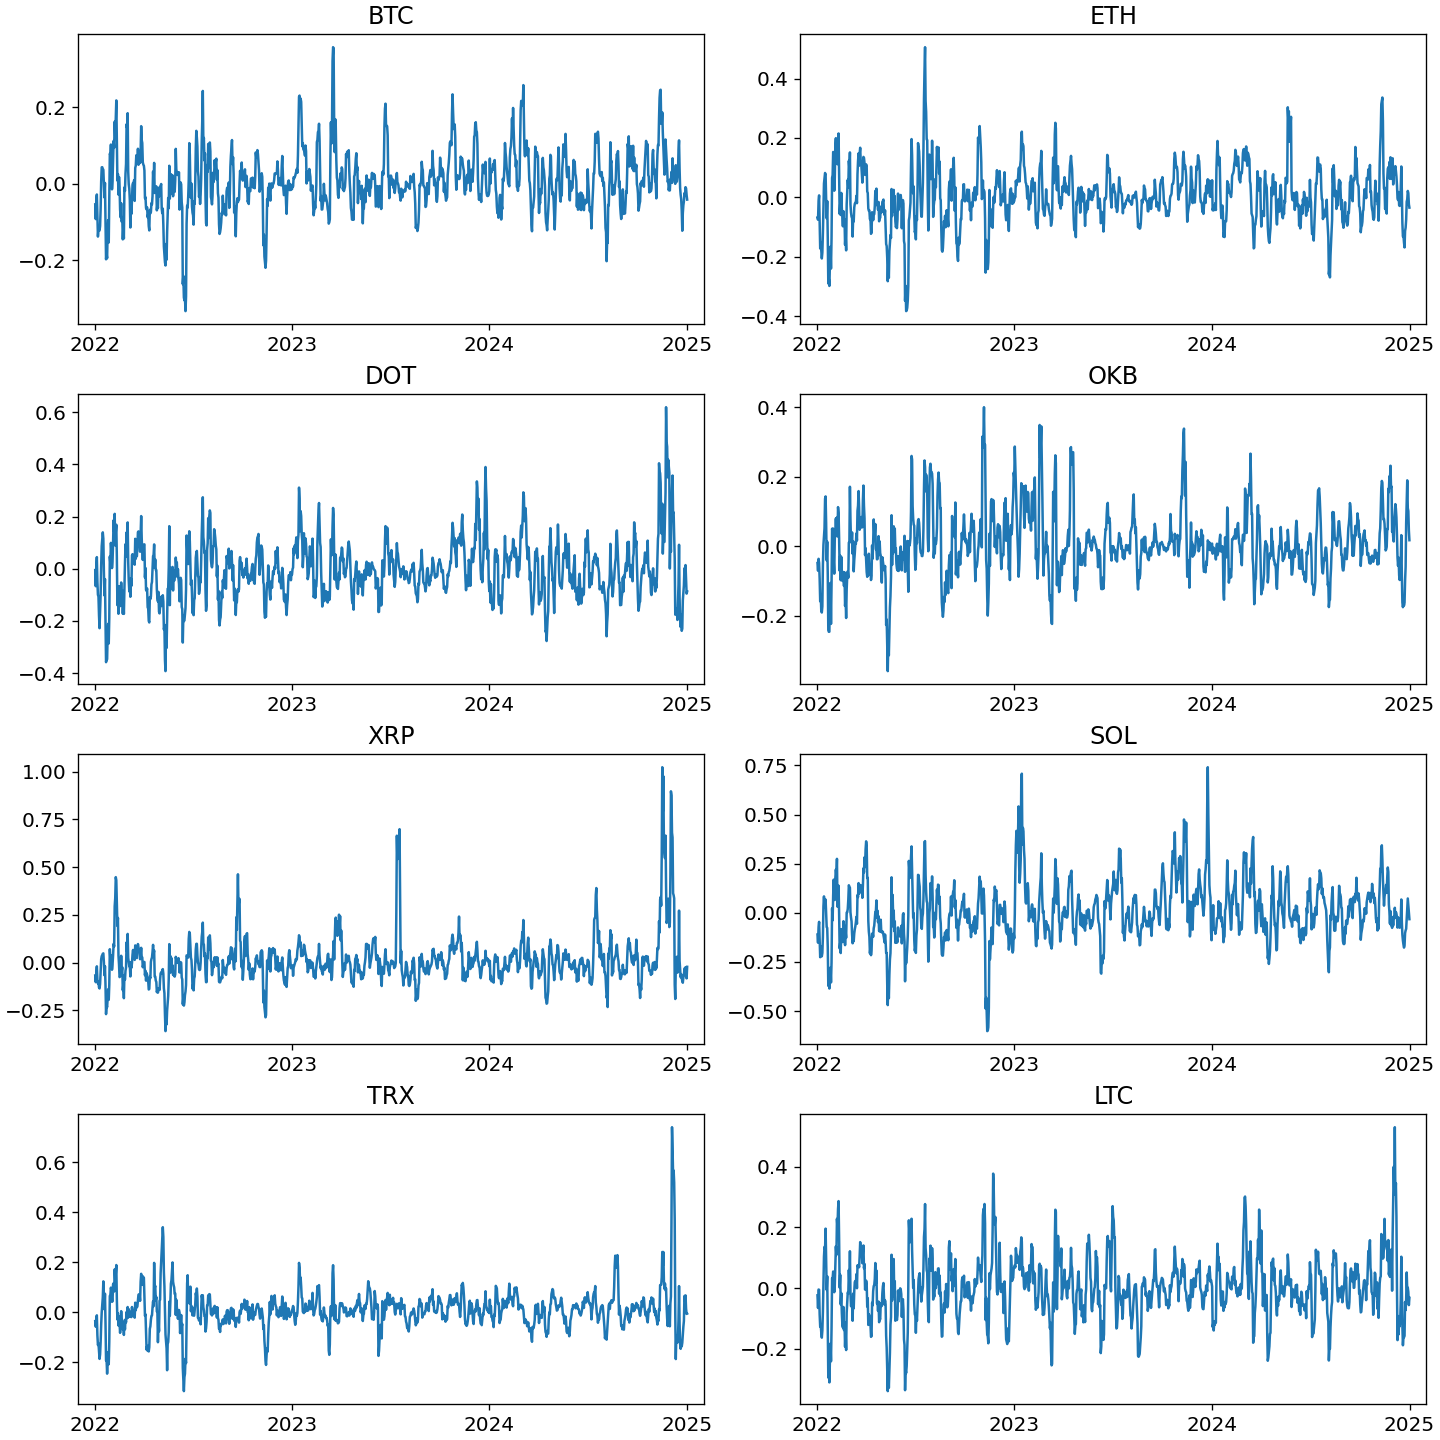
\includegraphics[width=1\textwidth]{returns.png}
                \caption{Доходности активов}
                \label{fig:returns}
            \end{figure}
        \end{column}
    \end{columns}
\end{frame}

\begin{frame}
    \frametitle{}
    \begin{table}[h]
        \caption{Доходности активов}
        \setlength{\tabcolsep}{3pt}
        \begin{tabularx}{\textwidth}{lrrrrrrrr}
            \toprule
            & BTC & ETH & DOT & OKB & XRP & SOL & TRX & LTC \\
            \midrule
            mean & 0.0073 & 0.0038 & -0.0031 & 0.0077 & 0.0132 & 0.0114 & 0.0105 & 0.0025 \\
            std & 0.0779 & 0.0961 & 0.1110 & 0.0936 & 0.1328 & 0.1482 & 0.0800 & 0.1001 \\
            min & -0.3328 & -0.3830 & -0.3925 & -0.3591 & -0.3596 & -0.6018 & -0.3162 & -0.3392 \\
            25\% & -0.0358 & -0.0477 & -0.0724 & -0.0401 & -0.0506 & -0.0765 & -0.0236 & -0.0513 \\
            50\% & 0.0026 & -0.0013 & -0.0084 & -0.0016 & -0.0003 & -0.0034 & 0.0106 & 0.0001 \\
            75\% & 0.0446 & 0.0555 & 0.0573 & 0.0494 & 0.0430 & 0.0906 & 0.0373 & 0.0546 \\
            max & 0.3566 & 0.5056 & 0.6188 & 0.4003 & 1.0235 & 0.7409 & 0.7407 & 0.5294 \\
            \bottomrule
        \end{tabularx}
        \label{tab:returns_describe}
    \end{table}
\end{frame}

\begin{frame}
    \frametitle{}
    \begin{figure}[H]
        \centering
        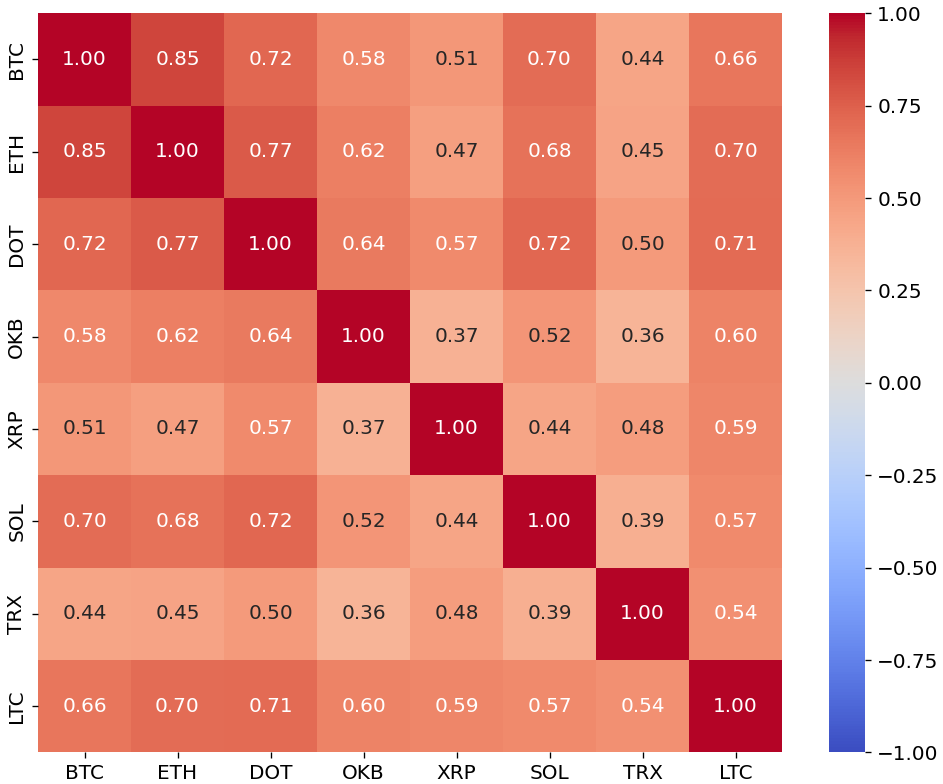
\includegraphics[width=0.8\textwidth]{corr_cut.png}
        \caption{Корреляции доходностей активов}
        \label{fig:corr}
    \end{figure}
\end{frame}

\subsection{Оценка средних доходностей}

\begin{frame}
    \frametitle{Модели оценки средней доходности $\hat{\mu}$}
    \begin{enumerate}
        \item NAIVE --- среднее выборочное
        \item MARTINGAL --- последнее наблюдаемое
        \item ARIMA --- модель ARIMA
        \item LR --- линейная регрессия
        \item RF --- случайный лес
    \end{enumerate}

    Качество прогнозирования оценивается по метрике 
    \[
	MSE = \frac{1}{n} \sum_{i=1}^{n} (\mu_i - \hat{\mu_i}_i)^2
    \]
    где $\mu_i$ - истинное значение доходности,
    а $\hat{\mu}_i$ - прогнозное значение модели на $i$-м объекте тестовой выборки.
\end{frame}

\begin{frame}
    \begin{table}[h]
    \caption{Качество прогнозирования, MSE$\cdot 10^4$}
        \label{tab:ml_eval_metrics}
        \begin{tabular}{lrrrrr}
            \toprule
            & NAIVE & MARTINGAL & LR & ARIMA & RF \\
            \midrule
            BTC & 5.63 & 1.20 & 1.58 & 1.62 & 2.07 \\
            ETH & 8.00 & 1.99 & 4.47 & 3.70 & 5.05 \\
            DOT & 16.51 & 3.89 & 4.09 & 3.98 & 5.28 \\
            OKB & 6.06 & 1.56 & 1.77 & 1.95 & 2.05 \\
            XRP & 24.33 & 5.04 & 6.98 & 5.71 & 6.53 \\
            SOL & 21.19 & 4.47 & 11.86 & 6.16 & 5.31 \\
            TRX & 7.96 & 1.85 & 4.19 & 5.30 & 6.04 \\
            LTC & 8.53 & 2.66 & 2.24 & 3.22 & 5.11 \\
            \bottomrule
        \end{tabular}
    \end{table}
\end{frame}

\subsection{Оценка ковариаций доходностей}

\begin{frame}
    \frametitle{Оценка матрицы ковариаций $\hat{\Sigma}$}
    Предполагается стационарность ковариаций во времени.

    Имея $r_t$ - вектор-столбец доходностей в момент времени t, по истории наблюдений $r_1, \cdots r_n$ 
    выборочная ковариация $\hat{\Sigma}$ рассчитывается как 
    \begin{align*}
        \hat{\Sigma} = \frac{1}{n} \sum_{t=1}^{n}(r_t - \overline{r}) \cdot (r_t - \overline{r})^T
    \end{align*}
    где $\overline{r} = \frac{1}{n} \sum_{t=1}^{n} r_t$.    
\end{frame}

\subsection{Результаты оценки стратегий}

\begin{frame}
    \frametitle{}
    \textbf{Стратегия} --- принцип по которому в каждый момент времени формируется портфель.

    Стратегии Марковица определяются моделью, лежащей в основе оценок $\hat{\mu}$ и $\hat{\Sigma}$,
    а так же зависят от параметра $\tau$.
    
    Тривиальные стратегии:
    \begin{enumerate}
        \item UNIFORM --- равномерное инвестирование во все активы
        \item MOST RISKY --- наиболее рискованный
        \item LESS RISKY --- наименее рискованный
        \item BEST RETURN --- с наибольшей доходностью
        \item WORST RETURN --- с наименьшей доходностью
    \end{enumerate}

    Доходность стратегии \textbf{ROI} (Return On Investment) определяется аналогично доходности портфеля.
\end{frame} 

\begin{frame}
    \begin{figure}
        \centering
        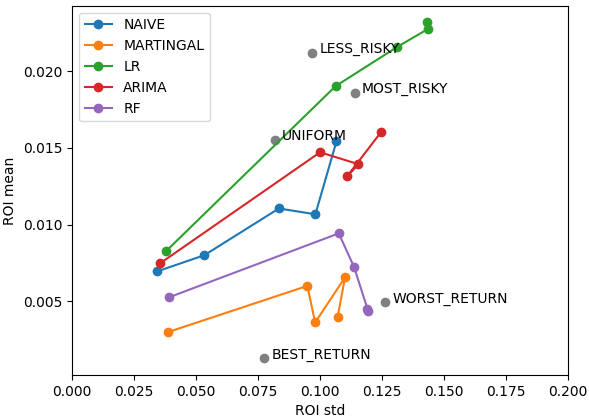
\includegraphics[width=0.9\textwidth]{result_frontiers_cut.png}
        \caption{Результаты тестирования стратегий}
        \label{fig:result_frontier}
    \end{figure}
\end{frame}

\begin{frame}
    \frametitle{}
    \begin{table}[H]
        \caption{Тривиальные портфели}
        \label{tab:trivial_rois}
        \begin{tabular}{lrr}
            \toprule
            & mean ROI $\cdot 10^3$ & std ROI $\cdot 10^2$ \\
            \midrule
            UNIFORM & 15.5372 & 8.1775 \\
            MOST RISKY & 18.5904 & 11.3970 \\
            LESS RISKY & 21.1635 & 9.6881 \\
            BEST RETURN & 1.2790 & 7.7329 \\
            WORST RETURN & 4.9217 & 12.6324 \\
            \bottomrule
        \end{tabular}
    \end{table}
\end{frame}

\begin{frame}
    \begin{table}[H]
        \caption{Средние ROI $\cdot 10^3$}
        \label{tab:roi_mean}
        \begin{tabular}{lrrrrr}
            \toprule
            &  0.01 &  0.25 &  0.50 &  0.75 &  1.00 \\
            \midrule
            NAIVE & 6.9451 & 8.0025 & 11.0462 & 10.6657 & 15.4227 \\
            MARTINGAL & 2.9859 & 6.0019 & 3.6178 & 6.5656 & 3.9942 \\
            LR & 8.2600 & 19.0185 & 21.5537 & 22.7442 & 23.1668 \\
            ARIMA & 7.4648 & 14.7066 & 13.9296 & 13.1520 & 15.9971 \\
            RF & 5.2633 & 9.4236 & 7.2398 & 4.3777 & 4.5050 \\
            \bottomrule
        \end{tabular}
    \end{table}
\end{frame}

\begin{frame}
    \begin{table}[H]
        \caption{Стандартное отклонение ROI $\cdot 10^2$}
        \label{tab:roi_std}
        \begin{tabular}{lrrrrr}
            \toprule
            &  0.01 &  0.25 &  0.50 &  0.75 &  1.00 \\
            \midrule
            NAIVE & 3.4328 & 5.3375 & 8.3427 & 9.8131 & 10.6650 \\
            MARTINGAL & 3.8577 & 9.4886 & 9.8051 & 11.0111 & 10.7128 \\
            LR & 3.7892 & 10.6314 & 13.1000 & 14.3570 & 14.3071 \\
            ARIMA & 3.5454 & 10.0037 & 11.5506 & 11.1001 & 12.4518 \\
            RF & 3.9215 & 10.7564 & 11.3710 & 11.9397 & 11.9118 \\
            \bottomrule
        \end{tabular}
    \end{table}
\end{frame}

\section{Выводы}

\begin{frame}
    \frametitle{Выводы}
    \begin{itemize}
        \item активы имеют сильную положительную корреляцию
        \item стремление сформировать портфель с большей доходностью влечет большие риски
        \item диверсификация действительно позволяет снижать риск портфеля
        \item как правило, формирование портфеля доминирует над инвестированием в отдельные активы
        \item линейная модель авторегрессии показала лучшее качество для оценки средней доходности
    \end{itemize}
\end{frame}

\begin{frame}
    \frametitle{Дальнейшие шаги}
    \begin{itemize}
        \item рассмотреть другие классы методов прогнозирования временных рядов
        \item помимо авторегрессионных признаков, учесть влияние внешних факторов на формирование цен
        \item расширить рассматриваемый набор активов
        \item исследовать другие таймфреймы и периоды инвестирования
    \end{itemize}
\end{frame}

\begin{frame}
    \frametitle{Использованные источники}
    \begin{enumerate}
        \item 
        Библиотека Python для прогнозирования временных рядов с использованием моделей машинного обучения
        [Электронный ресурс]. --- Режим доступа: https://skforecast.org/0.15.1/. --- Дата доступа 25.05.2025

        \item 
        Библиотека машинного обучения с открытым исходным кодом.
        [Электронный ресурс]. --- Режим доступа: https://scikit-learn.org/stable/. --- Дата доступа 25.05.2025
        
        \item 
        Криптовалютная биржа с расширенными финансовыми предложениями
        [Электронный ресурс]. --- 
        Режим доступа: https://www.okx.com/. --- Дата доступа: 25.05.2025

        \item 
        Шарп, У.Ф. Инвестиции : учебник : пер. с англ. / У.Ф. Шарп, Г.Д. Александер, Д.В. Бэйли. -- Москва : ИНФРА-М,, 2022. -- 1028 с.

        \item 
        Ширяев, А. Н. Основы стохастической финансовой математики: Т.1: Факты, модели / А. Н. Ширяев -- МЦНМО, 2016. -- 440 с.

        \item 
        Ширяев, А. Н. Основы стохастической финансовой математики: Т.2: Теория / А. Н. Ширяев -- МЦНМО, 2016. -- 464 с.
    \end{enumerate}
\end{frame}

\begin{frame}
    \frametitle{Использованные источники}
    \begin{enumerate}
        \setcounter{enumi}{6}
        \item 
        Breiman, L. Random Forests. Machine Learning / Leo Breiman --- 
        Statistics Department University of California Berkele, CA, 2001, 33 p.
        
        \item 
        Markowitz, H. Portfolio selection / 
        H. Markowitz --- The Journal of Finance, March 1952, 77-91 p.

        \item 
        Linter J. The valuation of risky assets and the selection of risky investments on stock portfolios and capital budgets /
        John Linter --- Review of Economics and Statistics, February 1965, 13-34 p.

        \item 
        Nakamoto S. Bitcoin: A Peer-to-Peer Electronic Cash System / 
        Satoshi Nakamoto --- Japan, 2008, 9 p.
        
        \item 
        Roll R., Ross S. A. An emperical investigation of the arbitrage pricing theory /
        Richard Roll, Stephen Ross --- Journal of Finance, 1980, 1073-1103 p.

        \item 
        Ross S. A. The arbitrage theory of capital asset pricing /
        Stephen A. Ross --- Journal of Finance, 1989, 1-18 p.
        
        \item 
        Sharpe W. F. Capital asset prices: A theory of market equilibrium under conditions of risk /
        William F. Sharp --- Journal of Finance, September 1964, 425-442 p.
    \end{enumerate}
\end{frame}

\begin{frame}
    \centering
    Спасибо за внимание.
\end{frame}

\end{document}